% ============================================================
% FEE3411 Control Systems A -- Lecture notes, Week 03
% Topic: Transfer functions and the s-plane
%
% Build:  latexmk -pdf week-03-notes.tex
% Needs:  ../tex/preamble.tex (this file lives in Notes/).
% ============================================================
\documentclass[11pt,a4paper]{article}
\usepackage[margin=25mm]{geometry}
% ============================================================
% FEE3411 Control Systems A -- shared preamble
% Used by both the lecture notes (article) and the slides (beamer).
% ============================================================
\usepackage[T1]{fontenc}
% lmodern gives cleaner PDF fonts but is absent from minimal TeX installs.
% Load it only if present, so this preamble builds anywhere.
\IfFileExists{lmodern.sty}{\usepackage{lmodern}}{}
\usepackage{amsmath,amssymb,amsthm}
\usepackage{graphicx}
\usepackage{booktabs}
\usepackage{siunitx}
\usepackage{tikz}
\usepackage{circuitikz}
\usepackage{pgfplots}
\pgfplotsset{compat=1.18}
\usetikzlibrary{arrows.meta,positioning,calc,decorations.markings,shapes.geometric}
\usepackage[most]{tcolorbox}
\usepackage{xcolor}

% ---- Course colours -------------------------------------------------
\definecolor{fnavy}{HTML}{1F3864}
\definecolor{faccent}{HTML}{2E5E4E}
\definecolor{fflag}{HTML}{9C4221}

% ---- Block-diagram style --------------------------------------------
\tikzset{
  block/.style   = {draw, thick, rectangle, minimum height=2.6em,
                    minimum width=3.2em, align=center},
  sumnode/.style = {draw, thick, circle, inner sep=0pt, minimum size=1.6em},
  pickoff/.style = {fill, circle, inner sep=0pt, minimum size=3pt},
  sig/.style     = {-{Latex[length=2mm]}, thick},
}

% ---- Summing-junction signs -----------------------------------------
% \sumsign{<node>}{<angle>}{<+ or ->} places a sign just outside the circle.
\newcommand{\sumsign}[3]{\node[font=\small] at ($(#1)+(#2:0.5)$) {$#3$};}

% ---- Boxed environments ---------------------------------------------
\newtcolorbox{keyidea}[1][]{colback=fnavy!5,colframe=fnavy,
  fonttitle=\bfseries,title=Key idea,#1}
\newtcolorbox{workedex}[1][]{colback=faccent!5,colframe=faccent,
  fonttitle=\bfseries,title=Worked example,#1}
\newtcolorbox{pitfall}[1][]{colback=fflag!5,colframe=fflag,
  fonttitle=\bfseries,title=Common pitfall,#1}

% ---- Shorthands ------------------------------------------------------
\newcommand{\Lap}{\mathcal{L}}
\newcommand{\jw}{\mathrm{j}\omega}
\newcommand{\wn}{\omega_{n}}
\newcommand{\zt}{\zeta}
\newcommand{\TF}[1]{#1(s)}

% ---- Week title machinery -------------------------------------------
\usepackage{fancyhdr}
\newcommand{\thecoursecode}{FEE3411}
\newcommand{\thecoursename}{Control Systems A}
\newcommand{\wknum}{}
\newcommand{\wktopic}{}
\newcommand{\weeknumber}[1]{\renewcommand{\wknum}{#1}}
\newcommand{\weektopic}[1]{\renewcommand{\wktopic}{#1}}
\newcommand{\weektitle}{%
  \thispagestyle{plain}%
  \begin{center}
    {\large\sffamily\bfseries\color{fnavy}\thecoursecode: \thecoursename}\\[2pt]
    {\Huge\sffamily\bfseries Week \wknum}\\[4pt]
    {\LARGE\sffamily\color{fnavy}\wktopic}\\[6pt]
    \rule{\textwidth}{1.2pt}
  \end{center}\vspace{4pt}%
  \pagestyle{fancy}\fancyhf{}%
  \fancyhead[L]{\footnotesize\color{gray}\thecoursecode\ Week \wknum\ --- \wktopic}%
  \fancyhead[R]{\footnotesize\color{gray}\thepage}%
  \renewcommand{\headrulewidth}{0.4pt}%
}

% ---- Outcomes and reading boxes -------------------------------------
\newenvironment{outcomes}
  {\begin{tcolorbox}[colback=white,colframe=fnavy!60,
      fonttitle=\bfseries,title=By the end of this week you should be able to]
   \begin{itemize}[leftmargin=*]}
  {\end{itemize}\end{tcolorbox}}

\newtcolorbox{readingbox}{colback=gray!5,colframe=gray!50,
  fonttitle=\bfseries,title=Reading}

% enumitem must NOT be loaded under beamer: it overwrites beamer's itemize
% templates and the bullet markers silently disappear. The notes (article) get
% it; the slides (beamer) use beamer's own list machinery instead.
\makeatletter
\@ifclassloaded{beamer}{}{\usepackage{enumitem}}
\makeatother


\weeknumber{3}
\weektopic{Transfer Functions and the $s$-Plane}

\begin{document}
\weektitle

% --------------------------------------------------------------------
\section*{What this week covers}

\begin{outcomes}
\item Solve a linear constant-coefficient differential equation with non-zero
      initial conditions by Laplace transform, and separate the forced response
      from the natural response in the answer.
\item Define the transfer function of an LTI system and derive it directly from
      the system differential equation, stating the zero-initial-condition
      assumption that makes the definition legitimate.
\item Obtain a transfer function of an electrical network in one step using
      the impedances $R$, $Ls$ and $1/Cs$, without first writing a differential
      equation.
\item Find the poles and zeros of a transfer function, draw its pole--zero map,
      and read the form of the natural response off the pole locations alone.
\item Invert a rational transfer function by partial fractions for distinct
      real poles and for a complex-conjugate pair.
\item Explain what a zero does to a response --- and what it does not do ---
      including the initial undershoot of a non-minimum-phase system.
\item Compute the d.c.\ gain of a transfer function and state the condition
      under which the final value theorem may be applied at all.
\item State the discrete-time counterparts of the transfer function and of the
      stability region, and write the transfer function of a pure time delay,
      distinguishing it from the transient specification called delay time.
\end{outcomes}

\begin{readingbox}
\textbf{Primary} --- Khalil, \S2-1 Differential Equation and Transfer Function
Models (pp.~10--14); Appendix~A, Review of the Laplace Transform (p.~438);
Appendix~C, Laplace and $z$-Transform Tables (p.~444).\\
\textbf{Secondary} --- Nise (6th ed.), \S2.3 The Transfer Function (p.~44);
\S4.2 Poles, Zeros, and System Response (p.~162); \S10.12 Systems with Time
Delay (p.~597, concept only --- the Bode treatment there belongs to Week~10).\\
\textbf{Further} --- Sundararajan, \S2.1--2.3.
\end{readingbox}

\noindent
\emph{Contact hours this week:} 2\,h lecture $+$ 1\,h tutorial.\\
\emph{Syllabus items addressed:} ``Laplace transform solution to a linear
constant-coefficient differential equation. Transfer functions as developed
from system differential equations. Definitions and properties in the
$s$-plane.'' (Transfer Functions); ``Continuous and discrete time-invariant
systems. Delay time.'' (Time Domain Linear Systems Analysis); ``Pole-zero
map'' (S-Domain Analysis).\\
\emph{Expected learning outcomes:} ELO~2 --- \emph{analyse a control system
solution in the time- and frequency-domains}; ELO~4 --- \emph{analyse the
stability of a control system} (the pole-location picture built here is the
stability picture used from Week~7 onward).

\bigskip
\noindent
\textbf{A note on the two halves.} The first lecture hour is about getting a
transfer function: the Laplace transform as a method of solving differential
equations, the definition of the transfer function, and the impedance shortcut
that was promised at the end of Week~2. The second hour is about reading one:
poles, zeros, the pole--zero map, d.c.\ gain, and the two extensions the
syllabus asks for --- discrete-time systems and pure time delay. Week~2 built
models; this week turns them into the object that every remaining week of
FEE3411 operates on.

% ====================================================================
\part*{Part A --- From differential equation to transfer function}
\addcontentsline{toc}{part}{Part A}

% --------------------------------------------------------------------
\section{Why the Laplace transform}
\label{sec:laplace}

Week~2 ended with differential-equation models. Solving them in the time domain
means finding a complementary function, finding a particular integral, and
fixing constants from initial conditions --- a different piece of work for every
new input. The Laplace transform replaces all of that with algebra.

The (one-sided) Laplace transform of $f(t)$ is
\begin{equation}
  F(s) = \Lap\{f(t)\} = \int_{0^-}^{\infty} f(t)\,e^{-st}\,dt ,
  \label{eq:laplace-def}
\end{equation}
where $s=\sigma+\jw$ is a complex variable (Khalil, p.~438). The lower limit is
written $0^-$, just \emph{before} $t=0$, so that an impulse applied at the
origin is captured rather than half-captured. Table~\ref{tab:pairs} lists the
pairs and properties used in this unit; Khalil's Appendix~C (p.~444) is the
fuller table to work from.

\begin{table}[htbp]
\centering
\caption{Laplace transform pairs and properties used in FEE3411.
Cf.\ Khalil, App.~C, p.~444.}
\label{tab:pairs}
\small
\begin{tabular}{@{}llll@{}}
\toprule
\multicolumn{2}{@{}l}{\textbf{Pairs}} & \multicolumn{2}{l@{}}{\textbf{Properties}}\\
$f(t),\ t\ge0$ & $F(s)$ & & \\
\midrule
$\delta(t)$              & $1$                              & Linearity        & $\alpha f_1+\beta f_2 \ \to\ \alpha F_1+\beta F_2$\\
$1(t)$ (unit step)       & $1/s$                            & First derivative & $\dot f \ \to\ sF(s)-f(0^-)$\\
$t$                      & $1/s^{2}$                        & Second derivative& $\ddot f \ \to\ s^{2}F(s)-sf(0^-)-\dot f(0^-)$\\
$e^{-at}$                & $1/(s+a)$                        & Integral         & $\int_{0}^{t}\!f \ \to\ F(s)/s$\\
$t e^{-at}$              & $1/(s+a)^{2}$                    & Time shift       & $f(t-\tau)1(t-\tau)\ \to\ e^{-\tau s}F(s)$\\
$\sin\omega t$           & $\omega/(s^{2}+\omega^{2})$      & Frequency shift  & $e^{-at}f(t)\ \to\ F(s+a)$\\
$\cos\omega t$           & $s/(s^{2}+\omega^{2})$           & Initial value    & $f(0^{+})=\lim_{s\to\infty}sF(s)$\\
$e^{-at}\sin\omega t$    & $\omega/[(s+a)^{2}+\omega^{2}]$  & Final value      & $f(\infty)=\lim_{s\to0}sF(s)$, \emph{if stable}\\
$e^{-at}\cos\omega t$    & $(s+a)/[(s+a)^{2}+\omega^{2}]$   & Convolution      & $f_1*f_2 \ \to\ F_1F_2$\\
\bottomrule
\end{tabular}
\end{table}

The derivative properties are the ones that do the work. Because
$\Lap\{\dot f\}=sF(s)-f(0^-)$ and $\Lap\{\ddot f\}=s^2F(s)-sf(0^-)-\dot f(0^-)$,
transforming a differential equation turns every derivative into a power of $s$
and every initial condition into an additive constant. What was a differential
equation in $t$ becomes a polynomial equation in $s$, which is solved by
rearrangement.

\begin{keyidea}
The transform does three things at once: it turns differentiation into
multiplication by $s$, it turns convolution into multiplication, and it carries
the initial conditions into the algebra automatically instead of leaving them
to be fitted at the end. The price is that the answer comes back in the
$s$-domain and has to be inverted --- which is what \S\ref{sec:partial} is
about.
\end{keyidea}

% --------------------------------------------------------------------
\section{Solving a linear constant-coefficient ODE}
\label{sec:ode-solution}

The procedure is mechanical:

\begin{enumerate}[leftmargin=*]
\item Transform every term of the differential equation, keeping the initial
      conditions.
\item Collect the terms in $Y(s)$ and solve for $Y(s)$ --- ordinary algebra.
\item Split $Y(s)$ into partial fractions.
\item Invert term by term using Table~\ref{tab:pairs}.
\end{enumerate}

\begin{workedex}[breakable, title=Worked example 3.1 --- an ODE with non-zero initial conditions]
Solve
\[
  \ddot y + 3\dot y + 2y = 2u(t), \qquad u(t)=1(t), \qquad
  y(0^-)=2, \quad \dot y(0^-)=0 .
\]

\textbf{Step 1 --- transform.} Using the derivative properties,
\[
  \bigl[s^{2}Y - s\,y(0^-) - \dot y(0^-)\bigr]
  + 3\bigl[sY - y(0^-)\bigr] + 2Y = \frac{2}{s} .
\]
Substituting $y(0^-)=2$ and $\dot y(0^-)=0$,
\[
  s^{2}Y - 2s + 3sY - 6 + 2Y = \frac{2}{s} .
\]

\textbf{Step 2 --- solve for $Y(s)$.}
\[
  Y(s)\,(s^{2}+3s+2) = \frac{2}{s} + 2s + 6
  \qquad\Longrightarrow\qquad
  Y(s) = \underbrace{\frac{2}{s(s+1)(s+2)}}_{\text{forced}}
       + \underbrace{\frac{2s+6}{(s+1)(s+2)}}_{\text{natural}} .
\]
Note that $s^{2}+3s+2=(s+1)(s+2)$ is the \emph{characteristic polynomial} of
Week~2 --- it appears as the denominator of both terms, whatever the input and
whatever the initial conditions.

\textbf{Step 3 --- partial fractions.} Term by term,
\[
  \frac{2}{s(s+1)(s+2)} = \frac{1}{s} - \frac{2}{s+1} + \frac{1}{s+2},
  \qquad
  \frac{2s+6}{(s+1)(s+2)} = \frac{4}{s+1} - \frac{2}{s+2},
\]
so that
\[
  Y(s) = \frac{1}{s} + \frac{2}{s+1} - \frac{1}{s+2} .
\]

\textbf{Step 4 --- invert.}
\[
  \boxed{\,y(t) = 1 + 2e^{-t} - e^{-2t}\,}, \qquad t\ge 0 .
\]

\textbf{Check.} $y(0)=1+2-1=2$ \checkmark;\ \ $\dot y(0)=-2+2=0$ \checkmark;\ \
$y(\infty)=1$, the steady state the step input should produce. The constant
term is the \emph{forced} response; the two exponentials, whose rates $-1$ and
$-2$ are the roots of the characteristic equation, are the \emph{natural}
response.
\end{workedex}

Two features of that answer are general and worth stating separately. The
\emph{shape} of the natural response --- which exponentials appear --- is set
by the characteristic equation, that is, by the plant. The \emph{size} of each
term is set by the input and the initial conditions. This separation is the
whole reason the $s$-plane picture in Part~B is useful.

% --------------------------------------------------------------------
\section{The transfer function}
\label{sec:tf}

Initial conditions describe how the system happened to be started, not what the
system \emph{is}. To characterise the system itself, set them all to zero.

\begin{keyidea}
The \textbf{transfer function} $G(s)$ of an LTI system is the ratio of the
Laplace transform of the output to the Laplace transform of the input, with all
initial conditions zero:
\[
  G(s) = \frac{Y(s)}{U(s)}\bigg|_{\text{zero initial conditions}} .
\]
It is a property of the system alone. It does not depend on the input, and it
does not depend on how the system was started.
\end{keyidea}

Applying this to the general model of Week~2,
\[
  a_n y^{(n)} + \cdots + a_1\dot y + a_0 y
  = b_m u^{(m)} + \cdots + b_1\dot u + b_0 u ,
\]
every derivative becomes a power of $s$ with no leftover constants, so
\begin{equation}
  G(s) = \frac{Y(s)}{U(s)}
       = \frac{b_m s^{m} + b_{m-1}s^{m-1} + \cdots + b_1 s + b_0}
              {a_n s^{n} + a_{n-1}s^{n-1} + \cdots + a_1 s + a_0}
       = \frac{N(s)}{D(s)} .
  \label{eq:tf-general}
\end{equation}
Reading \eqref{eq:tf-general} in reverse is just as useful: given a transfer
function, the differential equation can be written straight back down by
replacing $s^k Y$ with $y^{(k)}$ and $s^k U$ with $u^{(k)}$.

\begin{figure}[htbp]
\centering
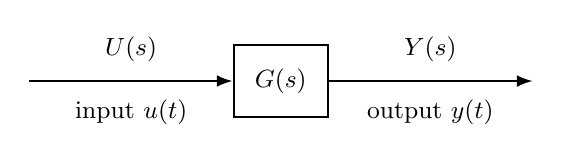
\begin{tikzpicture}[x=1cm,y=1cm,font=\small]
\node[block, minimum width=3.4em] (G) at (0,0) {$G(s)$};
\draw[sig] (-3.2,0) -- (G.west);
\draw[sig] (G.east) -- (3.2,0);
\node[above,font=\small] at (-1.9,0.12) {$U(s)$};
\node[below,font=\small] at (-1.9,-0.12) {input $u(t)$};
\node[above,font=\small] at (1.9,0.12) {$Y(s)$};
\node[below,font=\small] at (1.9,-0.12) {output $y(t)$};
\end{tikzpicture}
\caption{The transfer function as a block: $Y(s)=G(s)\,U(s)$. Multiplication in
the $s$-domain replaces convolution in the time domain. Cf.\ Nise Fig.~2.2,
p.~45.}
\label{fig:tf-block}
\end{figure}

Several properties follow immediately from \eqref{eq:tf-general}, and each is
used later in the unit:

\begin{itemize}[leftmargin=*]
\item \textbf{The denominator is the characteristic polynomial.} Setting
      $D(s)=0$ gives the characteristic equation of Week~2. Every stability
      method from Week~7 onward is a statement about the roots of $D(s)$.
\item \textbf{Order.} The order of the system is $n$, the degree of $D(s)$.
\item \textbf{Proper and strictly proper.} A physical system has $m\le n$
      (\emph{proper}); most have $m<n$ (\emph{strictly proper}). A transfer
      function with $m>n$ would differentiate its input more times than it
      integrates, which no physical device does. The difference $n-m$ is the
      \textbf{relative degree}, and \S\ref{sec:zeros} shows it is visible in
      the very first instant of the step response.
\item \textbf{The impulse response.} Since $\Lap\{\delta(t)\}=1$, the response
      to a unit impulse is $Y(s)=G(s)$, so $g(t)=\Lap^{-1}\{G(s)\}$. The
      transfer function \emph{is} the impulse response, transformed.
\item \textbf{Series connection.} Two blocks in cascade multiply:
      $Y=G_2G_1U$. This is the property Week~4 builds block-diagram algebra on.
\end{itemize}

\begin{pitfall}
The zero-initial-condition assumption is part of the definition, not an
approximation --- but it does not mean initial conditions are unimportant. When
a problem gives non-zero initial conditions, go back to the method of
\S\ref{sec:ode-solution}; the transfer function alone cannot express them. A
transfer function tells you how the system responds to an \emph{input}, not how
it decays from a \emph{state}.
\end{pitfall}

% --------------------------------------------------------------------
\section{Worked example: the series $RLC$ network}
\label{sec:rlc}

Week~2 derived the differential equation of the series $RLC$ network of
Figure~\ref{fig:rlc}(a) from Kirchhoff's voltage law:
\[
  LC\,\ddot v_o + RC\,\dot v_o + v_o = v_i .
\]

\begin{figure}[htbp]
\centering
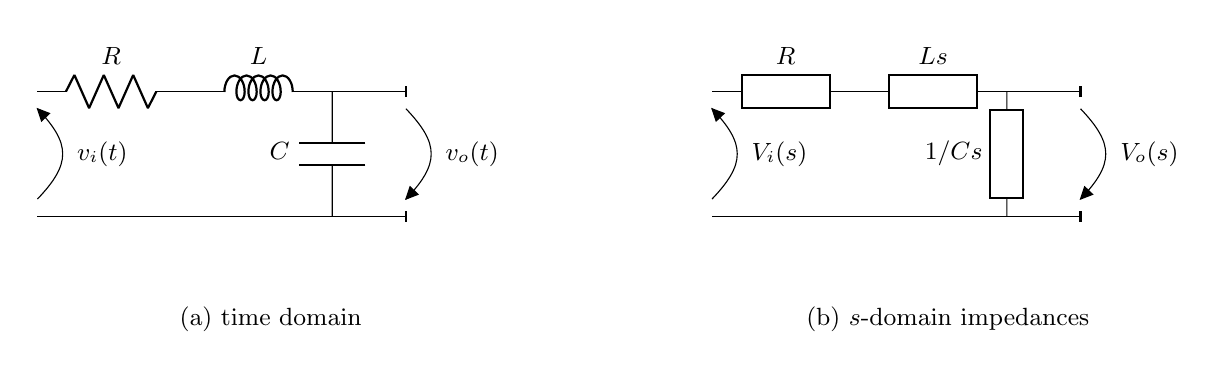
\begin{tikzpicture}
\node at (0,0) {%
\begin{circuitikz}[scale=0.72, every node/.style={font=\small}]
\draw (0,0) to[R=$R$] (2.6,0) to[L=$L$] (5.2,0);
\draw (5.2,0) to[C, l_=$C$] (5.2,-2.2);
\draw (5.2,-2.2) -- (0,-2.2);
\draw (0,0) to[open, v^<=$v_i(t)$] (0,-2.2);
\draw[thick] (6.5,-0.1) -- (6.5,0.1);
\draw[thick] (6.5,-2.3) -- (6.5,-2.1);
\draw (5.2,0) -- (6.5,0);
\draw (5.2,-2.2) -- (6.5,-2.2);
\draw (6.5,0) to[open, v^>=$v_o(t)$] (6.5,-2.2);
\end{circuitikz}};
\node at (8.6,0) {%
\begin{circuitikz}[scale=0.72, every node/.style={font=\small}]
\draw (0,0) to[generic=$R$] (2.6,0) to[generic=$Ls$] (5.2,0);
\draw (5.2,0) to[generic, l_=$1/Cs$] (5.2,-2.2);
\draw (5.2,-2.2) -- (0,-2.2);
\draw (0,0) to[open, v^<=$V_i(s)$] (0,-2.2);
\draw[thick] (6.5,-0.1) -- (6.5,0.1);
\draw[thick] (6.5,-2.3) -- (6.5,-2.1);
\draw (5.2,0) -- (6.5,0);
\draw (5.2,-2.2) -- (6.5,-2.2);
\draw (6.5,0) to[open, v^>=$V_o(s)$] (6.5,-2.2);
\end{circuitikz}};
\node[font=\small] at (0,-2.4) {(a) time domain};
\node[font=\small] at (8.6,-2.4) {(b) $s$-domain impedances};
\end{tikzpicture}
\caption{The series $RLC$ network of Week~2, drawn (a) with its components and
(b) with their $s$-domain impedances. The output is the capacitor voltage in
both. Cf.\ Khalil Fig.~2-4, p.~17.}
\label{fig:rlc}
\end{figure}

\begin{workedex}[breakable, title=Worked example 3.2 --- transfer function of the series $RLC$ network]
With zero initial conditions, transform the differential equation directly:
\[
  LCs^{2}V_o(s) + RCsV_o(s) + V_o(s) = V_i(s)
  \qquad\Longrightarrow\qquad
  \boxed{\ \frac{V_o(s)}{V_i(s)} = \frac{1}{LCs^{2}+RCs+1}\ } .
\]
Take $R=\SI{3}{\ohm}$, $L=\SI{1}{\henry}$, $C=\SI{0.5}{\farad}$. Then
$LC=0.5$ and $RC=1.5$, so
\[
  G(s) = \frac{1}{0.5s^{2}+1.5s+1}
       = \frac{2}{s^{2}+3s+2}
       = \frac{2}{(s+1)(s+2)} .
\]
The characteristic equation is $s^{2}+3s+2=0$, with roots $s=-1$ and $s=-2$:
two distinct, real, negative roots, so the natural response is the sum of two
decaying exponentials and there is no oscillation. The d.c.\ gain is
$G(0)=2/2=1$, so a constant input is passed through unchanged in the steady
state --- as it must be, since in steady state the inductor is a short circuit
and the capacitor an open circuit, and the whole source voltage appears across
$C$.
\end{workedex}

% --------------------------------------------------------------------
\section{The impedance shortcut}
\label{sec:impedance}

Week~2 promised that the differential equation could be skipped entirely for an
electrical network. Here is why. Transforming the element relations of Week~2
with zero initial conditions gives
\[
  V_R(s) = R\,I(s), \qquad
  V_L(s) = Ls\,I(s), \qquad
  V_C(s) = \frac{1}{Cs}\,I(s),
\]
so each element obeys $V=ZI$ --- Ohm's law, with a complex \textbf{impedance}
$Z$ in place of a resistance:
\[
  Z_R = R, \qquad Z_L = Ls, \qquad Z_C = \frac{1}{Cs} .
\]

\begin{keyidea}
Impedances in series add, and impedances in parallel combine as reciprocals,
exactly as resistances do. So an $s$-domain network can be reduced by the
ordinary rules of resistive circuit analysis --- voltage dividers, current
dividers, series/parallel combination --- and the transfer function drops out
without a differential equation ever being written.
\end{keyidea}

For Figure~\ref{fig:rlc}(b), the output is taken across $Z_C$ in a series loop,
so the voltage divider gives the result in one line:
\[
  \frac{V_o(s)}{V_i(s)} = \frac{Z_C}{Z_R+Z_L+Z_C}
  = \frac{1/Cs}{R+Ls+1/Cs}
  = \frac{1}{LCs^{2}+RCs+1},
\]
in agreement with Worked example~3.2. The same shortcut generalises to any
network: write Kirchhoff's laws in the $s$-domain with impedances and solve the
resulting algebraic equations. Week~4 will use it constantly.

\begin{pitfall}
The impedance shortcut is only valid with \emph{zero initial conditions} ---
no initial inductor current, no initial capacitor charge. That is exactly the
condition under which a transfer function is defined, so for transfer-function
work the shortcut is always available. If a question gives an initial capacitor
voltage and asks for the full response, the shortcut does not apply and the
method of \S\ref{sec:ode-solution} is required.
\end{pitfall}

% ====================================================================
\part*{Part B --- Reading a transfer function: the $s$-plane}
\addcontentsline{toc}{part}{Part B}

% --------------------------------------------------------------------
\section{Poles, zeros and the pole--zero map}
\label{sec:polezero}

Write the transfer function in factored form:
\begin{equation}
  G(s) = K\,\frac{(s-z_1)(s-z_2)\cdots(s-z_m)}{(s-p_1)(s-p_2)\cdots(s-p_n)} .
  \label{eq:factored}
\end{equation}

\begin{itemize}[leftmargin=*]
\item The \textbf{zeros} $z_1,\dots,z_m$ are the roots of the numerator: the
      values of $s$ at which $G(s)=0$.
\item The \textbf{poles} $p_1,\dots,p_n$ are the roots of the denominator: the
      values of $s$ at which $G(s)$ becomes infinite. They are the roots of the
      characteristic equation.
\item $K$ is the \textbf{gain factor}. It is \emph{not} the d.c.\ gain ---
      see \S\ref{sec:dcgain}.
\end{itemize}

Because the coefficients of $N(s)$ and $D(s)$ are real, any complex poles or
zeros occur in conjugate pairs, so the pole--zero map is always symmetric about
the real axis. Plotting poles as $\times$ and zeros as $\circ$ on the complex
plane gives the \textbf{pole--zero map}, and that picture is essentially the
whole of the system's dynamics.

\begin{figure}[htbp]
\centering
\begin{tikzpicture}[x=0.95cm,y=0.62cm,font=\small]
% axes
\draw[->,thick] (-4.6,0) -- (1.6,0) node[right] {$\sigma$};
\draw[->,thick] (0,-4.3) -- (0,4.3) node[above] {$\jw$};
% ticks: only where no marker sits, so nothing is drawn through a symbol
\foreach \x in {-4,-2} \draw (\x,0.16) -- (\x,-0.16) node[below,font=\scriptsize] {$\x$};
\foreach \y/\l in {3/3,-3/-3} \draw (0.06,\y) -- (-0.06,\y) node[left,font=\scriptsize] {$\l$};
% poles (crosses), drawn with a white disc behind so the axis does not show through
\foreach \py in {0,3,-3}{%
  \fill[white] (-1,\py) circle (0.2);
  \draw[thick,fnavy] (-1.16,\py-0.24) -- (-0.84,\py+0.24);
  \draw[thick,fnavy] (-1.16,\py+0.24) -- (-0.84,\py-0.24);}
% zero (circle), likewise
\fill[white] (-3,0) circle (0.2);
\draw[thick,fflag] (-3,0) circle (0.17);
% labels: all placed to the LEFT of their markers, well clear of the imaginary axis
\node[fnavy,font=\scriptsize,left] at (-1.35,0.75) {$p_1=-1$};
\node[fnavy,font=\scriptsize,left] at (-1.35,3) {$p_2=-1+\mathrm{j}3$};
\node[fnavy,font=\scriptsize,left] at (-1.35,-3) {$p_3=-1-\mathrm{j}3$};
\node[fflag,font=\scriptsize,below] at (-3,-1.35) {$z_1=-3$};
\end{tikzpicture}
\caption{Pole--zero map of
$G(s)=4(s+3)/\bigl[(s+1)(s^{2}+2s+10)\bigr]$: poles ($\times$) at $-1$ and
$-1\pm\mathrm{j}3$, a zero ($\circ$) at $-3$. Cf.\ Nise \S4.2, p.~162.}
\label{fig:pzmap}
\end{figure}

% --------------------------------------------------------------------
\section{The poles set the natural modes}
\label{sec:modes}

Partial-fraction expansion of $Y(s)=G(s)U(s)$ produces one term for each pole.
Each term inverts to a characteristic function of time, called a \textbf{mode},
and the pole's position in the plane fixes which function it is. Real part
$\sigma$ controls growth or decay; imaginary part $\omega$ controls
oscillation. Table~\ref{tab:modes} is the dictionary.

\begin{table}[htbp]
\centering
\caption{Pole location and the mode it contributes to the natural response.}
\label{tab:modes}
\small
\renewcommand{\arraystretch}{1.5}
\begin{tabular}{@{}p{4.1cm}p{4.3cm}c@{}}
\toprule
\textbf{Pole location} & \textbf{Term in $y(t)$} & \textbf{Shape}\\
\midrule
Negative real, $s=-a$ & $Ae^{-at}$, decaying &
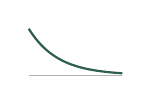
\begin{tikzpicture}[baseline=0.3cm,x=0.22cm,y=0.28cm]
\draw[gray!60] (0,0) -- (5.4,0); \draw[thick,faccent] plot[domain=0:5.4,samples=40] (\x,{2.1*exp(-0.6*\x)});
\end{tikzpicture}\\
At the origin, $s=0$ & $A$, constant (an integrator) &

\begin{tikzpicture}[baseline=0.3cm,x=0.22cm,y=0.28cm]
\draw[gray!60] (0,0) -- (5.4,0); \draw[thick,faccent] (0,1.5) -- (5.4,1.5);
\end{tikzpicture}\\
Positive real, $s=+a$ & $Ae^{+at}$, growing &
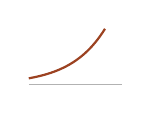
\begin{tikzpicture}[baseline=0.3cm,x=0.22cm,y=0.28cm]
\draw[gray!60] (0,0) -- (5.4,0); \draw[thick,fflag] plot[domain=0:4.4,samples=40] (\x,{0.28*exp(0.5*\x)});
\end{tikzpicture}\\
Complex pair, $s=-a\pm\jw$ & $Ae^{-at}\sin(\omega t+\phi)$, damped oscillation &
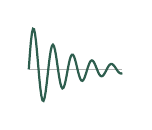
\begin{tikzpicture}[baseline=0.3cm,x=0.22cm,y=0.28cm]
\draw[gray!60] (0,0) -- (5.4,0); \draw[thick,faccent] plot[domain=0:5.4,samples=90] (\x,{2.1*exp(-0.45*\x)*sin(320*\x)});
\end{tikzpicture}\\
Pair on the $\jw$ axis, $s=\pm\jw$ & $A\sin(\omega t+\phi)$, sustained &
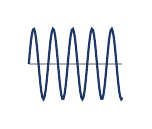
\begin{tikzpicture}[baseline=0.3cm,x=0.22cm,y=0.28cm]
\draw[gray!60] (0,0) -- (5.4,0); \draw[thick,fnavy] plot[domain=0:5.4,samples=90] (\x,{1.6*sin(320*\x)});
\end{tikzpicture}\\
Complex pair, $s=+a\pm\jw$ & $Ae^{+at}\sin(\omega t+\phi)$, growing &
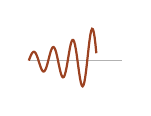
\begin{tikzpicture}[baseline=0.3cm,x=0.22cm,y=0.28cm]
\draw[gray!60] (0,0) -- (5.4,0); \draw[thick,fflag] plot[domain=0:3.9,samples=80] (\x,{0.36*exp(0.38*\x)*sin(320*\x)});
\end{tikzpicture}\\
\bottomrule
\end{tabular}
\end{table}

The pattern in Table~\ref{tab:modes} has one consequence large enough to
organise the rest of the unit around.

\begin{keyidea}
Every mode decays if and only if its pole has a \emph{strictly negative real
part}. So an LTI system is stable exactly when all of its poles lie in the open
left half of the $s$-plane. A single pole in the right half plane, however
small the rest of the system's margins, makes the whole response grow without
bound.
\end{keyidea}

\begin{figure}[htbp]
\centering
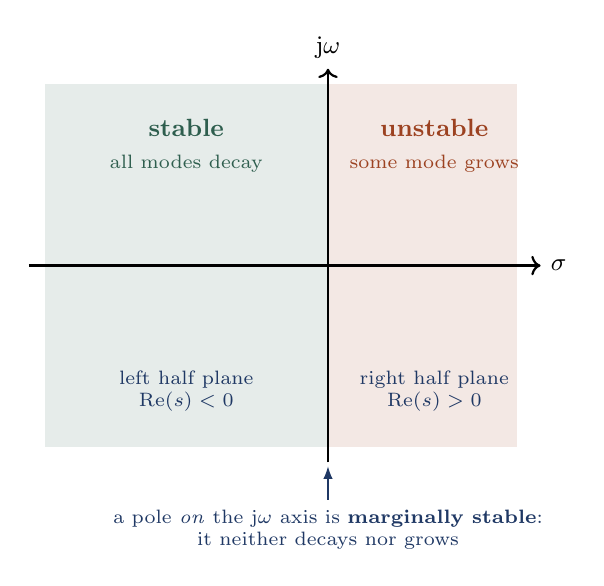
\begin{tikzpicture}[x=1cm,y=1cm,font=\small]
\fill[faccent!12] (-3.6,-2.3) rectangle (0,2.3);
\fill[fflag!12] (0,-2.3) rectangle (2.4,2.3);
\draw[->,thick] (-3.8,0) -- (2.7,0) node[right] {$\sigma$};
\draw[->,thick] (0,-2.5) -- (0,2.5) node[above] {$\jw$};
\node[faccent,font=\small\bfseries] at (-1.8,1.75) {stable};
\node[faccent,font=\scriptsize] at (-1.8,1.3) {all modes decay};
\node[fflag,font=\small\bfseries] at (1.35,1.75) {unstable};
\node[fflag,font=\scriptsize] at (1.35,1.3) {some mode grows};
\node[fnavy,font=\scriptsize,align=center] at (-1.8,-1.6)
  {left half plane\\ $\mathrm{Re}(s)<0$};
\node[fnavy,font=\scriptsize,align=center] at (1.35,-1.6)
  {right half plane\\ $\mathrm{Re}(s)>0$};
% annotation for the boundary, placed below the axes and pointing up at it
\node[fnavy,font=\scriptsize,align=center] (marg) at (0,-3.35)
  {a pole \emph{on} the $\jw$ axis is \textbf{marginally stable}:\\
   it neither decays nor grows};
\draw[fnavy,-{Latex[length=1.6mm]}] (marg.north) -- (0,-2.55);
\end{tikzpicture}
\caption{The stability picture in the $s$-plane. Every stability test in
Weeks~7--12 --- Routh--Hurwitz, root locus, Nyquist --- is a different way of
answering the same question: are any poles to the right of the imaginary axis?}
\label{fig:splane-regions}
\end{figure}

% --------------------------------------------------------------------
\section{Inverse Laplace by partial fractions}
\label{sec:partial}

Getting from $Y(s)$ back to $y(t)$ means splitting $Y(s)$ into terms that
appear in Table~\ref{tab:pairs}. Three cases cover everything met in this unit.

\paragraph{Distinct real poles.} Write one term per pole and find each residue
by the cover-up rule: multiply through by that factor and evaluate at the pole.
This is the case of Worked example~3.1.

\paragraph{Repeated poles.} A factor $(s+a)^{r}$ needs $r$ terms,
$A_1/(s+a)+A_2/(s+a)^2+\cdots+A_r/(s+a)^r$, and inverts to terms in
$e^{-at}$, $te^{-at}$, \dots, $t^{r-1}e^{-at}$.

\paragraph{Complex-conjugate poles.} A quadratic factor
$s^{2}+2\zt\wn s+\wn^{2}$ that does not factor over the reals is best kept
whole and matched to the last two pairs of Table~\ref{tab:pairs} by completing
the square, rather than split into two complex terms.

\begin{workedex}[breakable, title=Worked example 3.3 --- a complex-pole step response]
Find the unit-step response of
\[
  G(s) = \frac{10}{s^{2}+2s+10} .
\]

\textbf{Poles.} $s = \dfrac{-2\pm\sqrt{4-40}}{2} = -1\pm\mathrm{j}3$: a complex
pair in the left half plane, so the response is a damped oscillation. Comparing
with $s^{2}+2\zt\wn s + \wn^{2}$ gives
$\wn=\sqrt{10}=\SI{3.16}{\radian\per\second}$ and
$\zt = 2/(2\wn) = 1/\sqrt{10}=0.316$ --- the notation of Week~5.

\textbf{Expand.} With $U(s)=1/s$,
\[
  Y(s) = \frac{10}{s\,(s^{2}+2s+10)} = \frac{1}{s} - \frac{s+2}{s^{2}+2s+10} .
\]

\textbf{Complete the square.} $s^{2}+2s+10=(s+1)^{2}+3^{2}$, so
\[
  \frac{s+2}{(s+1)^{2}+3^{2}}
  = \frac{(s+1)}{(s+1)^{2}+3^{2}} + \frac{1}{3}\cdot\frac{3}{(s+1)^{2}+3^{2}} ,
\]
which matches the $e^{-at}\cos\omega t$ and $e^{-at}\sin\omega t$ pairs with
$a=1$, $\omega=3$. Hence
\[
  \boxed{\ y(t) = 1 - e^{-t}\Bigl(\cos 3t + \tfrac{1}{3}\sin 3t\Bigr)\ },
  \qquad t\ge0 .
\]

\textbf{Check.} $y(0)=1-(1+0)=0$ \checkmark;\ \ $y(\infty)=1=G(0)$ \checkmark.
The envelope decays as $e^{-t}$, set by the real part of the poles; the
ringing is at $\SI{3}{\radian\per\second}$, set by the imaginary part.
\end{workedex}

\begin{pitfall}
Do not split a complex-conjugate pair into two separate first-order terms with
complex residues unless you intend to recombine them. It is legitimate, but the
algebra is error-prone and the answer arrives as a sum of complex exponentials
that still has to be turned back into a real sine and cosine. Completing the
square keeps everything real from start to finish.
\end{pitfall}

% --------------------------------------------------------------------
\section{What zeros do}
\label{sec:zeros}

Poles determine \emph{which} modes appear. Zeros do not create modes at all ---
they change how much of each mode appears, by changing the residues. The effect
is easiest to see by holding the poles and the d.c.\ gain fixed and moving a
single zero.

\begin{workedex}[breakable, title={Worked example 3.4 --- one zero, three systems}]
All three systems below have poles at $-1$ and $-2$ and d.c.\ gain $1$. They
differ only in their zero:
\[
  G_1(s) = \frac{2}{(s+1)(s+2)}, \qquad
  G_2(s) = \frac{2}{3}\,\frac{s+3}{(s+1)(s+2)}, \qquad
  G_3(s) = \frac{2}{3}\,\frac{3-s}{(s+1)(s+2)} .
\]
$G_1$ has no zero; $G_2$ has a zero at $s=-3$ (left half plane); $G_3$ has a
zero at $s=+3$ (right half plane). Expanding each step response by partial
fractions:
\[
  y_1(t) = 1 - 2e^{-t} + e^{-2t}, \qquad
  y_2(t) = 1 - \tfrac{4}{3}e^{-t} + \tfrac{1}{3}e^{-2t}, \qquad
  y_3(t) = 1 - \tfrac{8}{3}e^{-t} + \tfrac{5}{3}e^{-2t} .
\]
The same two exponentials appear in all three --- only the coefficients differ.
Yet the responses behave very differently at the start:
\[
  \dot y_1(0)=0, \qquad \dot y_2(0)=+\tfrac{2}{3}, \qquad
  \dot y_3(0)=-\tfrac{2}{3} .
\]
$G_1$, with relative degree $2$, leaves the origin with zero slope. $G_2$ and
$G_3$, with relative degree $1$, leave with finite slope --- and $G_3$ leaves
in the \emph{wrong direction}, dipping to a minimum of $y_3=-1/15$ at
$t=\ln(5/4)=\SI{0.223}{\second}$ before recovering and settling at $1$.
\end{workedex}

\begin{figure}[htbp]
\centering
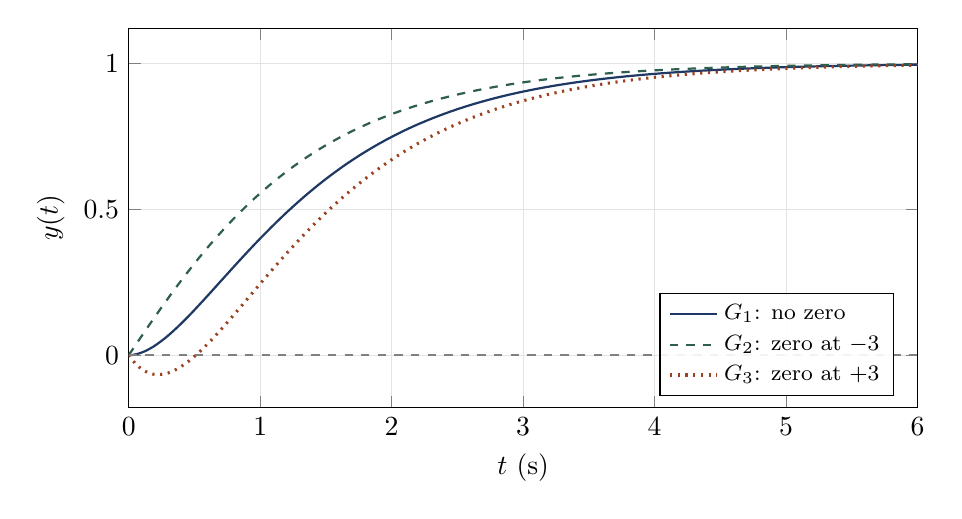
\begin{tikzpicture}
\begin{axis}[
  width=11.6cm, height=6.4cm,
  xlabel={$t$ (s)}, ylabel={$y(t)$},
  xmin=0, xmax=6, ymin=-0.18, ymax=1.12,
  grid=major, grid style={gray!22},
  legend pos=south east, legend cell align=left,
  legend style={font=\footnotesize, fill=white, fill opacity=0.9, text opacity=1},
  every axis plot/.append style={thick},
]
\addplot[domain=0:6, samples=200, fnavy] {1 - 2*exp(-x) + exp(-2*x)};
\addlegendentry{$G_1$: no zero}
\addplot[domain=0:6, samples=200, faccent, dashed] {1 - (4/3)*exp(-x) + (1/3)*exp(-2*x)};
\addlegendentry{$G_2$: zero at $-3$}
\addplot[domain=0:6, samples=200, fflag, dotted, line width=1.1pt] {1 - (8/3)*exp(-x) + (5/3)*exp(-2*x)};
\addlegendentry{$G_3$: zero at $+3$}
\addplot[gray, dashed, line width=0.5pt, forget plot] coordinates {(0,0) (6,0)};
\end{axis}
\end{tikzpicture}
\caption{Step responses of the three systems of Worked example~3.4. Identical
poles and identical d.c.\ gain; only the zero differs. The right-half-plane
zero of $G_3$ produces the initial undershoot.}
\label{fig:zeros}
\end{figure}

\begin{keyidea}
A zero adds no new mode and changes no time constant --- the exponentials are
the same in all three responses of Figure~\ref{fig:zeros}. What it changes is
the \emph{weighting} of the modes, and therefore the shape of the transient. A
zero in the right half plane produces an initial response in the wrong
direction; such a system is called \textbf{non-minimum-phase}.
\end{keyidea}

\begin{pitfall}
A right-half-plane \emph{zero} does not make a system unstable --- $G_3$
settles perfectly well at $1$. Only right-half-plane \emph{poles} cause
instability. What a right-half-plane zero does is make the system hard to
control, because feedback that reacts to the initial wrong-way motion pushes in
the wrong direction; this reappears in Week~8 as the characteristic shape of a
non-minimum-phase root locus.
\end{pitfall}

% --------------------------------------------------------------------
\section{D.c.\ gain and the final value theorem}
\label{sec:dcgain}

For a constant input, all derivatives vanish in the steady state, so $s\to0$
in the transfer function. The \textbf{d.c.\ gain} (or steady-state gain) is
\begin{equation}
  G(0) = \frac{b_0}{a_0} ,
  \label{eq:dcgain}
\end{equation}
the ratio of the constant terms. It is the factor by which a constant input is
multiplied once the transients have died away. For a unit step input, the
steady-state output \emph{is} $G(0)$.

The general statement is the final value theorem of Table~\ref{tab:pairs}:
\[
  y(\infty) = \lim_{s\to0} sY(s) = \lim_{s\to0} sG(s)U(s) .
\]
With $U(s)=1/s$ this reduces to $y(\infty)=G(0)$, as used to check every worked
example above.

\begin{pitfall}
The final value theorem is only valid if the final value \emph{exists} --- that
is, if all poles of $sY(s)$ lie strictly in the left half plane. Applied blindly
to the unstable system $G(s)=1/(s-1)$ it gives $y(\infty)=G(0)=-1$, whereas the
true step response is $y(t)=e^{t}-1$, which grows without bound. Check
stability first; the theorem cannot detect its own misuse.
\end{pitfall}

Note also that the gain factor $K$ of the factored form \eqref{eq:factored} is
not the d.c.\ gain. For $G_2$ of Worked example~3.4, $K=2/3$ but
$G_2(0)=\tfrac{2}{3}\cdot\tfrac{3}{2}=1$. Multiplying the poles and zeros back
in is the only safe way to get the steady-state gain.

% --------------------------------------------------------------------
\section{Discrete time-invariant systems}
\label{sec:discrete}

Everything so far assumes a signal defined for every instant $t$. A digital
controller instead sees samples $u[k]=u(kT)$ at a sampling period $T$, and its
model is a \textbf{difference} equation rather than a differential one:
\[
  y[k] + \alpha_1 y[k-1] + \cdots + \alpha_n y[k-n]
  = \beta_0 u[k] + \cdots + \beta_m u[k-m] .
\]
The $z$-transform, $Y(z)=\sum_{k=0}^{\infty}y[k]z^{-k}$, plays exactly the role
the Laplace transform plays for continuous signals. Its key property is the
shift rule: with zero initial conditions, a one-step delay $y[k-1]$ transforms
to $z^{-1}Y(z)$. So a delay becomes multiplication by $z^{-1}$, just as
differentiation became multiplication by $s$, and the same argument as
\S\ref{sec:tf} gives a \textbf{pulse transfer function} $G(z)=Y(z)/U(z)$.

\begin{workedex}[breakable, title=Worked example 3.5 --- a first-order discrete system]
For $y[k] = 0.5\,y[k-1] + u[k]$, transforming with zero initial conditions
gives $Y(z)\bigl(1-0.5z^{-1}\bigr) = U(z)$, so
\[
  G(z) = \frac{1}{1-0.5z^{-1}} = \frac{z}{z-0.5},
\]
a single pole at $z=0.5$. The unit-step response is
$y[k] = 2 - (0.5)^{k}$, giving $1,\ 1.5,\ 1.75,\ 1.875,\dots$ and converging to
$G(1)=1/(1-0.5)=2$ --- the discrete d.c.\ gain, evaluated at $z=1$ rather than
$s=0$.
\end{workedex}

The stability region changes shape with the transform. A continuous mode
$e^{st}$ sampled at spacing $T$ becomes $z^{k}$ with $z=e^{sT}$, and that
mapping sends the left half plane to the interior of the unit circle.

\begin{keyidea}
A continuous system is stable when every pole satisfies $\mathrm{Re}(s)<0$;
a discrete system is stable when every pole satisfies $|z|<1$. Same idea,
different picture: the imaginary axis becomes the unit circle.
\end{keyidea}

\begin{figure}[htbp]
\centering
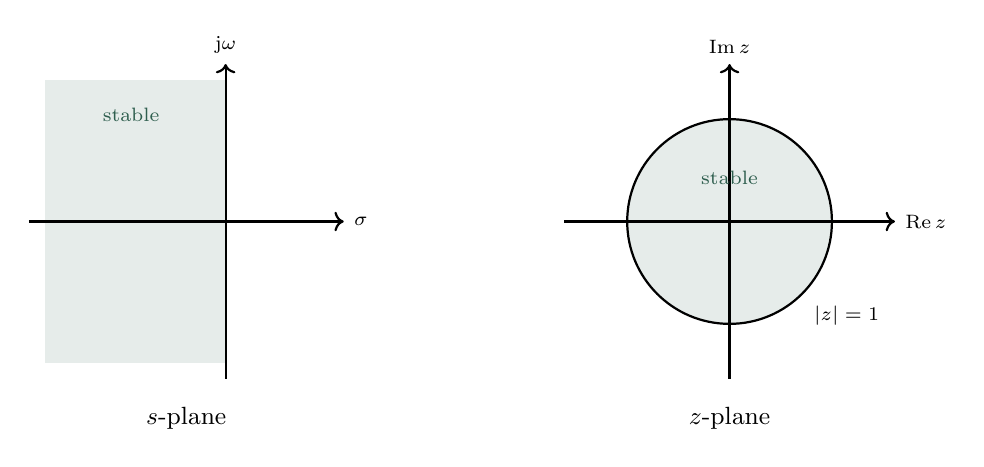
\begin{tikzpicture}[x=1cm,y=1cm,font=\small]
% s-plane
\begin{scope}
\fill[faccent!12] (-2.3,-1.8) rectangle (0,1.8);
\draw[->,thick] (-2.5,0) -- (1.5,0) node[right,font=\scriptsize] {$\sigma$};
\draw[->,thick] (0,-2.0) -- (0,2.0) node[above,font=\scriptsize] {$\jw$};
\node[font=\small] at (-0.5,-2.5) {$s$-plane};
\node[faccent,font=\scriptsize] at (-1.2,1.35) {stable};
\end{scope}
% z-plane
\begin{scope}[xshift=6.4cm]
\fill[faccent!12] (0,0) circle (1.3);
\draw[thick] (0,0) circle (1.3);
\draw[->,thick] (-2.1,0) -- (2.1,0) node[right,font=\scriptsize] {$\mathrm{Re}\,z$};
\draw[->,thick] (0,-2.0) -- (0,2.0) node[above,font=\scriptsize] {$\mathrm{Im}\,z$};
\node[font=\small] at (0,-2.5) {$z$-plane};
\node[faccent,font=\scriptsize] at (0,0.55) {stable};
\node[font=\scriptsize,below right] at (0.95,-0.95) {$|z|=1$};
\end{scope}
\end{tikzpicture}
\caption{Stability regions compared. The map $z=e^{sT}$ carries the shaded left
half plane onto the shaded interior of the unit circle.}
\label{fig:s-vs-z}
\end{figure}

FEE3411 works entirely in continuous time; this section exists because the
syllabus asks for the comparison, and because every controller you will
actually build is a discrete one running on a processor.

% --------------------------------------------------------------------
\section{Pure time delay, and delay time}
\label{sec:delay}

A conveyor belt, a length of pipe, a communication link and a computation all
introduce a \textbf{pure time delay} (or transport lag): the output is the
input, unchanged in shape, but later by $\tau$ seconds. By the time-shift
property of Table~\ref{tab:pairs},
\[
  y(t) = u(t-\tau)\,1(t-\tau)
  \qquad\Longrightarrow\qquad
  \frac{Y(s)}{U(s)} = e^{-\tau s} .
\]

\begin{figure}[htbp]
\centering
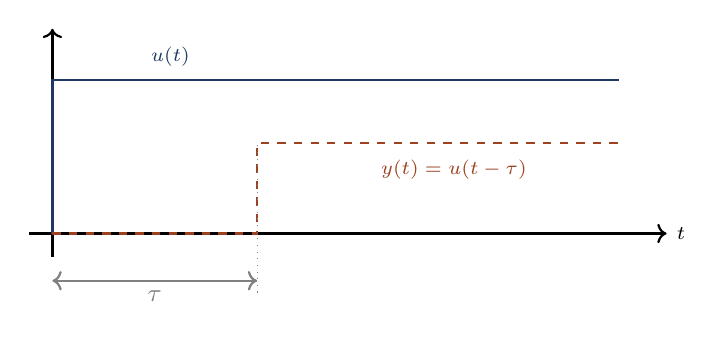
\begin{tikzpicture}[x=1cm,y=1cm,font=\small]
\draw[->,thick] (-0.3,0) -- (7.8,0) node[right,font=\scriptsize] {$t$};
\draw[->,thick] (0,-0.3) -- (0,2.6);
% input: steps up at t = 0
\draw[thick,fnavy] (0,0) -- (0,1.95) -- (7.2,1.95);
\node[fnavy,font=\scriptsize,above] at (1.5,2.0) {$u(t)$};
% output: the same step, tau seconds later, drawn lower so both stay visible
\draw[thick,fflag,dashed] (0,0) -- (2.6,0) -- (2.6,1.15) -- (7.2,1.15);
\node[fflag,font=\scriptsize,below] at (5.1,1.06) {$y(t)=u(t-\tau)$};
% the delay itself
\draw[gray,dotted] (2.6,-0.75) -- (2.6,1.15);
\draw[<->,thick,gray] (0,-0.6) -- (2.6,-0.6);
\node[gray,font=\small,below] at (1.3,-0.6) {$\tau$};
\end{tikzpicture}
\caption{A pure time delay reproduces the input shape exactly, $\tau$ seconds
later. (The two traces are drawn at slightly different heights only so that
both remain visible.)}
\label{fig:delay}
\end{figure}

\begin{pitfall}
$e^{-\tau s}$ is \emph{not} a rational function, so a system containing a pure
delay has no finite set of poles and zeros and cannot be drawn on a pole--zero
map. Every method in this unit that relies on a polynomial characteristic
equation --- Routh--Hurwitz in Week~7, root locus in Week~8 --- therefore does
not apply directly to a delay. The frequency-domain methods of Weeks~10--12 do,
because $e^{-\jw\tau}$ has magnitude~$1$ and phase $-\omega\tau$, which is
simply added to the phase plot. This is why Nise treats time delay in
\S10.12 (p.~597), inside the Bode chapter, rather than in the transfer-function
chapter.
\end{pitfall}

Where a rational approximation is needed, the \textbf{Pad\'e approximation}
supplies one. The first-order form (Khalil, p.~14) is
\begin{equation}
  e^{-\tau s} \approx \frac{1-\tau s/2}{1+\tau s/2} ,
  \label{eq:pade}
\end{equation}
whose series expansion agrees with $e^{-\tau s}$ up to and including the $s^{2}$
term. Notice where its zero sits: at $s=+2/\tau$, in the right half plane. A
delay behaves like a non-minimum-phase system in exactly the sense of
\S\ref{sec:zeros} --- which is the analytical reason delay is so damaging to a
feedback loop.

\begin{pitfall}
The syllabus phrase \emph{delay time} means something different from the pure
time delay $\tau$ of this section. Delay time $t_d$ is a transient
specification --- the time a step response takes to reach $50\%$ of its final
value --- and is defined in Week~5 for systems with no transport lag at all. A
system can have a delay time of \SI{0.4}{\second} and no time delay whatsoever.
Read which one a question means from its context.
\end{pitfall}

% --------------------------------------------------------------------
\section*{Summary}

\begin{itemize}
\item The Laplace transform turns a linear constant-coefficient differential
      equation into algebra, carrying initial conditions in automatically
      through $\Lap\{\dot f\}=sF(s)-f(0^-)$.
\item The transfer function $G(s)=Y(s)/U(s)$, defined with zero initial
      conditions, is a property of the plant alone. Its denominator is the
      characteristic polynomial, its inverse transform is the impulse response,
      and blocks in cascade multiply.
\item For an electrical network, the impedances $R$, $Ls$, $1/Cs$ give the
      transfer function directly by voltage- and current-divider algebra, with
      no differential equation.
\item Poles are the roots of the denominator, zeros the roots of the numerator;
      both are plotted on the pole--zero map, which is symmetric about the real
      axis.
\item Each pole contributes one mode: real part sets growth or decay, imaginary
      part sets oscillation. A system is stable exactly when every pole lies in
      the open left half plane.
\item Zeros add no modes; they reweight the residues and so reshape the
      transient. A right-half-plane zero causes initial undershoot
      (non-minimum-phase) but does not cause instability.
\item The d.c.\ gain is $G(0)=b_0/a_0$, and is not the gain factor $K$. The
      final value theorem gives it, but only for a stable system.
\item Discrete systems use $G(z)$ in place of $G(s)$, with the stability region
      the unit circle instead of the left half plane. A pure time delay has
      transfer function $e^{-\tau s}$, is not rational, and is distinct from
      the transient specification called delay time.
\end{itemize}

% --------------------------------------------------------------------
\section*{Before the tutorial}

\begin{enumerate}
\item Using impedances only, find $V_o(s)/V_i(s)$ for a series $RC$ network
      with the output taken across the resistor. Identify its pole, its zero
      and its d.c.\ gain, and say in one sentence what kind of filter it is.
\item A system has poles at $-2$ and $-5$, a zero at $-10$, and d.c.\ gain $3$.
      Write its transfer function in both factored and polynomial form, and
      state its relative degree.
\item Find the unit-step response of $G(s)=6/\bigl[(s+1)(s+3)\bigr]$ by partial
      fractions, and verify your answer at $t=0$ and $t\to\infty$.
\item Without computing anything, sketch the shape of the natural response of a
      system whose poles are at $-0.5\pm\mathrm{j}8$, and say which feature of
      the sketch is set by the $-0.5$ and which by the $8$.
\end{enumerate}

% --------------------------------------------------------------------
\section*{Looking ahead}

Week~4 keeps the transfer functions built here and asks how they combine when
subsystems are wired together: block-diagram representation, the canonical
feedback form, the reduction rules, and signal flow graphs with Mason's gain
formula. The impedance shortcut of \S\ref{sec:impedance} and the cascade rule
of \S\ref{sec:tf} are the two results Week~4 leans on hardest. Assignment~2,
issued at the start of Week~4 and due in Week~6, covers Weeks~3 and~4 together
--- so the partial-fraction and transfer-function work of this week is examined
alongside next week's material, and is worth consolidating now rather than
revisiting cold. Beyond that, the pole--zero map of \S\ref{sec:polezero} is the
picture the rest of the unit is drawn on: Week~5 reads transient specifications
off pole positions, Week~7 tests whether any pole has crossed into the right
half plane, and Week~8 tracks how the poles move as a gain is varied. Locating
those poles is \emph{analysis} and belongs here; choosing a compensator to put
them somewhere better is design, and belongs to FEE3412.

\end{document}
